%!TEX encoding=UTF-8 Unicode
%!TEX root=../tabarnac.tex

\section{Methodology of the Evaluation}
\label{sec:metho}

This section briefly discusses our evaluation methodology of \TABARNAC.
We present the hardware architecture and the applications that will be used in the analysis.

\subsection{Hardware Environment}
\label{sec:expe-setup}

\begin{table}[!b]
    \centering
    \caption{Hardware configuration of our evaluation system.}
    \label{tab:turing}
    \footnotesize
        \begin{tabular}{lccccc}
            \toprule
            \multirow{2}{1.5cm}{System total} & Nodes & Threads & Freq (GHz) & Memory (Gib) \\
            \cmidrule(lr){2-5}
                & $4$   & $64$ & $2.00$ & $128$ \\
            \midrule
           \multirow{2}{1.5cm}{\vspace{2mm}Per NUMA node} & Cores & Threads & L3 Cache (Mib) & Memory (GiB) \\
           \cmidrule(lr){2-5}
            & $8$ & $16$ & $18$ & $32$  \\
            \bottomrule
        \end{tabular}

\end{table}

All experiments were run on a NUMA machine that is composed of $4$ Intel Xeon X7550
processors (Nehalem microarchitecture~\cite{Intel2010}). Each processor has its own memory controller and therefore forms a NUMA node. The hardware details are summarized in Table~\ref{tab:turing}.
The machine runs version 3.13 of the Linux kernel.

For the plots representing speedups or execution time, each configuration was executed at least 10 times. Each point represents the arithmetic mean of all runs.
The error bars in those plots represent the standard deviation.

\subsection{Applications}

We evaluate the following applications with \TABARNAC: a \emph{matrix multiplication}, the \emph{IS} benchmark and \emph{Ondes3D}.
They were chosen to demonstrate different memory access behaviors with different strategies to improve them.

The \emph{matrix multiplication} is a well-known algorithm that is used to verify the accuracy of \TABARNAC, as well as to discuss the performance improvements that can be achieved.
\emph{IS} is a benchmark from the OpenMP implementation of the NAS Parallel Benchmark suite~(NPB)~\cite{Jin1999}. \emph{IS} sorts a set of integer numbers using a bucket sort algorithm.
\emph{Ondes3D} is the main numerical kernel of the Ondes3D application~\cite{Dupros2008}. It simulates the propagation of seismic waves using a finite-differences numerical method.
The \emph{matrix multiplication} is implemented with Pthreads, while \emph{IS} and \emph{Ondes3D} use OpenMP.

All applications were compiled with \texttt{gcc}, version 4.6.3, with the \texttt{-O2} optimization flag.
Due to space restrictions, we show the characterization of the applications
with 4 threads. However, the qualitative behavior remains the same with different numbers of threads. The performance evaluation is performed with 64 threads,
which is the maximum number of threads that our evaluation machine can execute
in parallel. The \emph{matrix multiplication} performance was evaluated with
matrices of size $4096 \times 4096$ doubles, for a memory usage of $12.8$Mib per matrix. \emph{IS} was run
with input class \emph{D}, resulting in a memory usage of $33.5$Gib, Finally, Ondes3D has a memory usage of $11.3$Gib.

\subsection{Mapping Policies}

In the performance evaluation, we compare the following traditional mapping policies to \TABARNAC.
The \emph{original Linux kernel} forms our baseline for the experiments. We use an unmodified Linux kernel, version 3.13, with the first-touch policy. The NUMA Balancing mechanism is disabled in this baseline.
The \emph{interleave} policy is performed with the help of the \texttt{numactl} tool.
We also compare our results to the recently introduced \emph{NUMA Balancing} technique~\cite{Corbet}, which is executed with its default configuration.


\section{Analysis and Performance Results}
\label{sec:expe-analysis}

This section presents the results of our analysis with \TABARNAC.
For each application, we show the memory access behavior, discuss strategies to optimize this behavior and present the performance improvements that can be achieved.

% In this section, we analyze several benchmarks using \TABARNAC, we discuss
% their memory access distribution. Using this analysis we propose some
% optimizations and we evaluate them by comparing it to automatic data mapping
% tools.

\subsection{Matrix Multiplication}
\label{sec:exp-mat}

The first benchmark presented is based on a naive matrix multiplication,
computing $C=A \times B$. Our aim here is not to provide a kernel competing with the
state of the art, but to show how \TABARNAC can help to improve such
applications. We compare two implementations of the matrix multiplication, in
the first one, called \emph{Naive}, each thread starts by computing
$C[0][tid]$ and then jumps $N$ elements after in the matrix, where $N$ is the
number of threads. Although this implementation is known to be inefficient, it is a
good example of NUMA-unaware code, and comparing the \TABARNAC visualization
for this algorithm to the one obtained with a better version helps understanding
how to interpret it.
The optimized implementation uses a non-recursive block
decomposition.
Moreover, when an application has such an unstructured memory access pattern, it
is not always possible to change the pattern completely. Therefore, it is
interesting to discuss the improvements we can obtain on this kernel without
modifying the algorithm.



\begin{figure}[!t]
    \centering
    \subfigure[Structure B (naive version).]{
        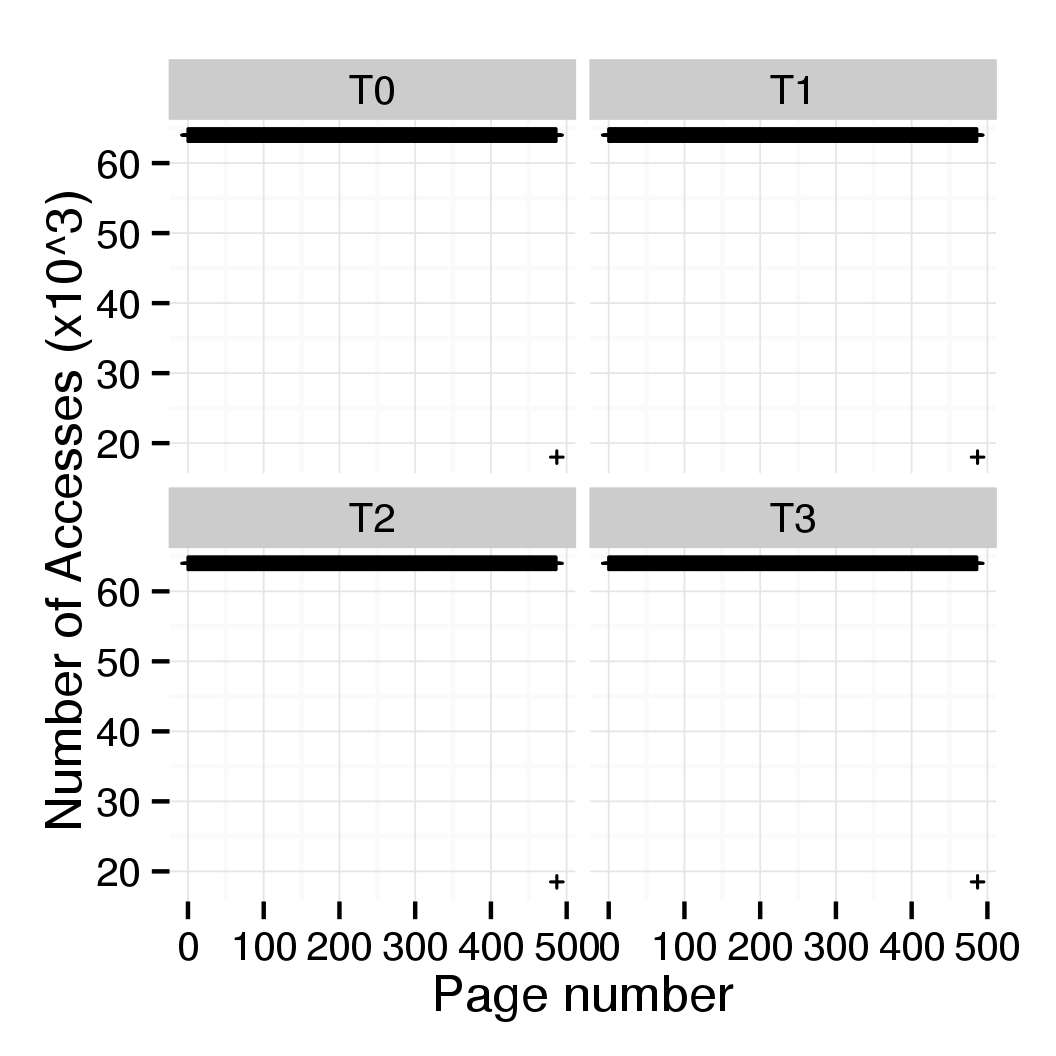
\includegraphics[width=.45\linewidth] {mat_B_modulo}
        \label{fig:matrix-B-naive}
    }
    \subfigure[Structure C (naive version).]{
        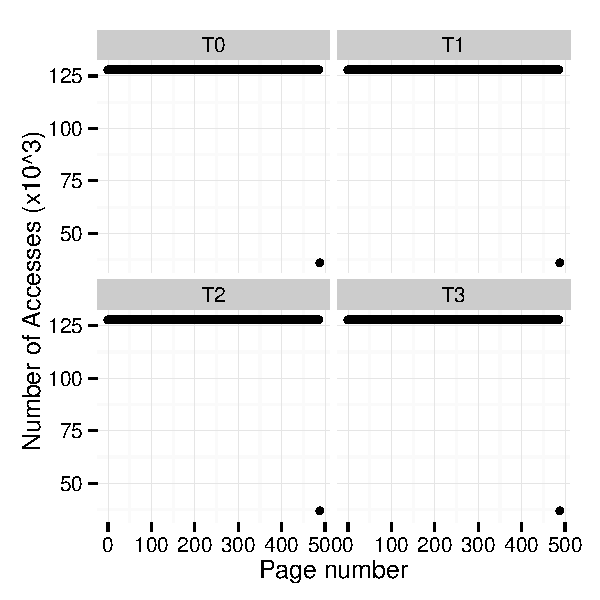
\includegraphics[width=.45\linewidth] {mat_C_modulo}
        \label{fig:matrix-C-naive}
    }
    \subfigure[Structure B (block version).]{
        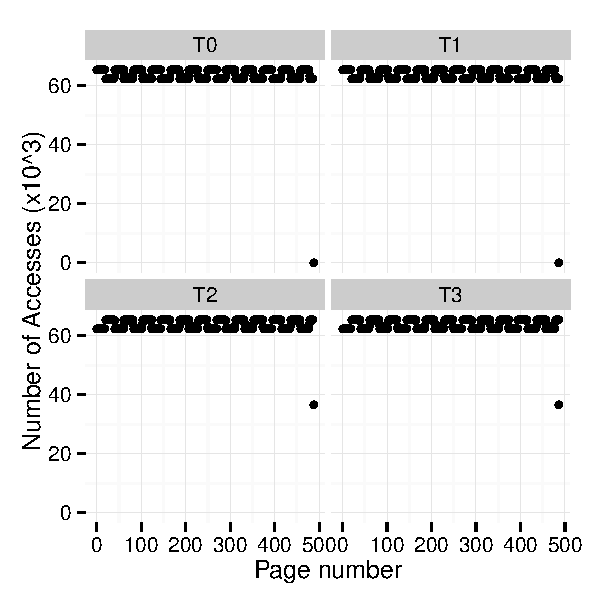
\includegraphics[width=.45\linewidth] {mat_B_bloc}
        \label{fig:matrix-B-bloc}
    }
    \subfigure[Structure C (block version).]{
        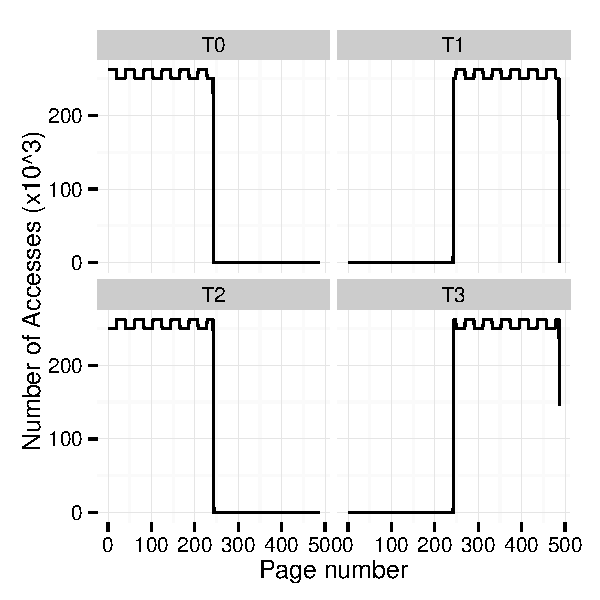
\includegraphics[width=.45\linewidth] {mat_C_bloc}
        \label{fig:matrix-C-bloc}
    }
    \caption{Per-thread access distribution on data structures B and C for the
    matrix multiplication.}
    \label{fig:matrix-analysis}
\end{figure}
% The figures presented in this sections are part of the \TABARNAC visualization.
The analysis of the matrix multiplication is shown in Figure~\ref{fig:matrix-analysis}.
Each plot shows the number of memory accesses for a particular data structure
per page and per thread. Only structures \texttt{B} and \texttt{C} are
presented, as for both algorithms \texttt{A} has a similar access
pattern as \texttt{C}.
For the naive matrix multiplication, as we can see in
Figures~\ref{fig:matrix-B-naive}~and~\ref{fig:matrix-C-naive}, all pages of both structures are used by every
thread. Therefore, when we execute this code on a NUMA machine, wherever we
map the page, all the nodes but one will trigger remote memory accesses. There
are several ways to improve this behavior: an easy solution
is to tell the operating system to interleave pages through the different
nodes. This will result in a better balance of memory bandwidth between the
nodes. Another solution is to create local copies of \texttt{A} and
\texttt{B} on each node as these matrices are only read. Finally, we can modify
the algorithm to improve the locality, which means using the block algorithm.

%\begin{figure}[htb]
%    \centering
%    \subfigure[Structure B (block version).]{
%        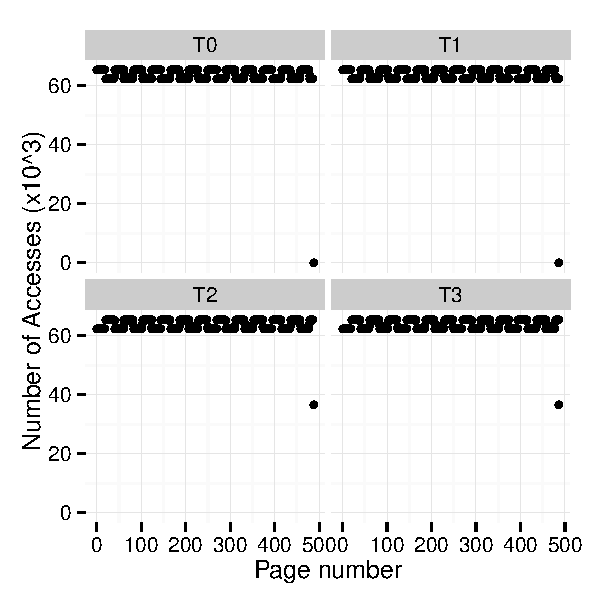
\includegraphics[height=.24\textheight] {mat_B_bloc}
%        \label{fig:matrix-B-bloc}
%    }
%    \subfigure[Structure C (block version).]{
%        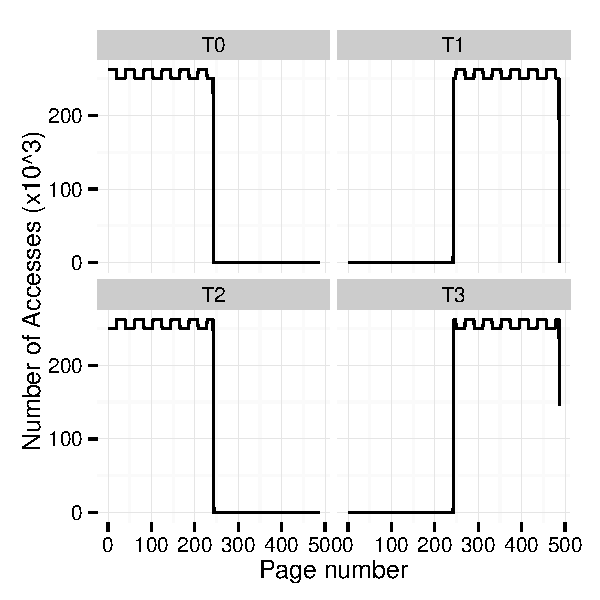
\includegraphics[height=.24\textheight] {mat_C_bloc}
%        \label{fig:matrix-C-bloc}
%    }
%    \caption{By thread access distribution on data structures A and B for the
%    block matrix multiplication.}
%    \label{fig:matrix-bloc}
%\end{figure}

As we can see in Figures~\ref{fig:matrix-B-bloc}~and~\ref{fig:matrix-C-bloc}, the block algorithm improves the page
locality compared to the naive implementation. In our algorithm, structures \texttt{B}
and \texttt{C} are not divided the same way, resulting in two different access patterns. For structure \texttt{B} (Figure~\ref{fig:matrix-B-bloc}), the pages still
have similar numbers of accesses for all threads. Structures \texttt{C} and
\texttt{A} (Figure~\ref{fig:matrix-C-bloc}) are split into two parts, the first half
is shared by threads $T0$ and $T2$ while the two others works on the second
half. This behavior provides strong page locality and is therefore more
suitable for NUMA machines. We can easily put each part of \texttt{C} (and
\texttt{A}) on a NUMA node and map the thread using it to this node, while matrix
\texttt{B} can be distributed using an interleave policy.

To evaluate the efficiency of the proposed modifications, we compare the execution
time of both versions of the code (naive and block) with the mapping suggested by \TABARNAC to the original Linux kernel (base), Interleave, and to NUMA Balancing.


\begin{figure}[!t]
    \centering
    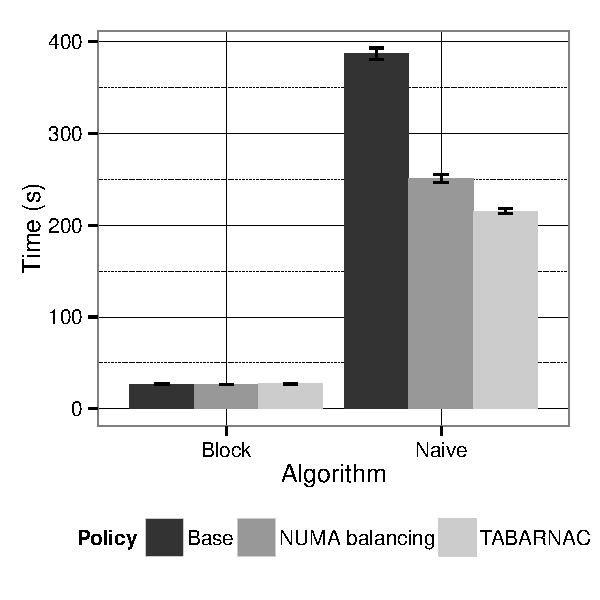
\includegraphics[width=.7\linewidth]{mat_time}
    \caption{Execution time of the matrix multiplication for size $4096\times 4096$ doubles.}
    \label{fig:matrix-res}
\end{figure}

Figure~\ref{fig:matrix-res} shows the experimental results of the matrix multiplication. We can see that for
the naive algorithm, NUMA Balancing is already quite efficient and results in $40\%$
speedup. However, using the \TABARNAC policy avoids the runtime overhead and
allows us to obtain almost $50\%$ of speedup. For the block version, all runtimes
provide the same execution time as this algorithm is designed to fit in the
caches of the system, such that the NUMA policy should not influence the results.

This example shows
how \TABARNAC can help improving an application by highlighting an inefficient
memory access behavior. This knowledge can be used two different ways, and always
results on significant improvement. Either the user can modify the code to
improve the access distribution (in this case going from the naive to the block version),
or at least \TABARNAC will help choosing the best NUMA page mapping policy.

\subsection{IS}
\label{sec:exp-is}

The \emph{IS} benchmark in its default version has an unstructured memory access behavior\footnote{\url{http://www.nas.nasa.gov/publications/npb.html}}. Thus, it is a good candidate to be optimized using \TABARNAC.
\begin{figure}[!p]
    \centering

    \subfigure[\texttt{key\_buff2}.]{
        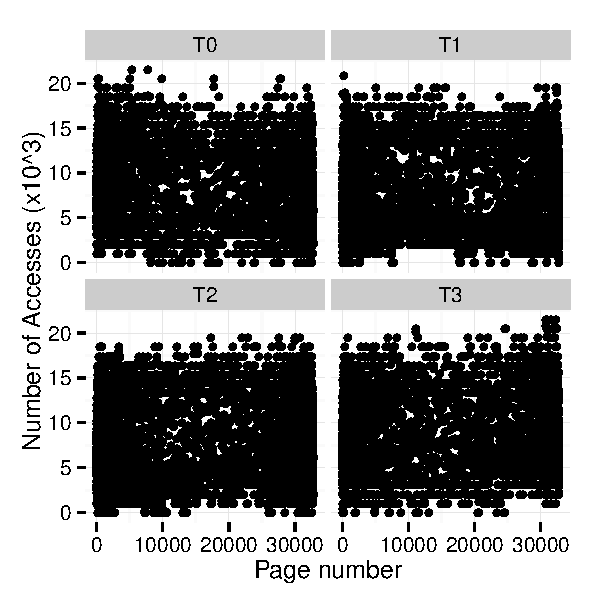
\includegraphics[height=.2\textheight]  {is_w_kb2_orig}
        \label{fig:is-behaviour-orig-kb2}
    }
    \vspace{-1mm}
    \subfigure[\texttt{key\_array}.]{
        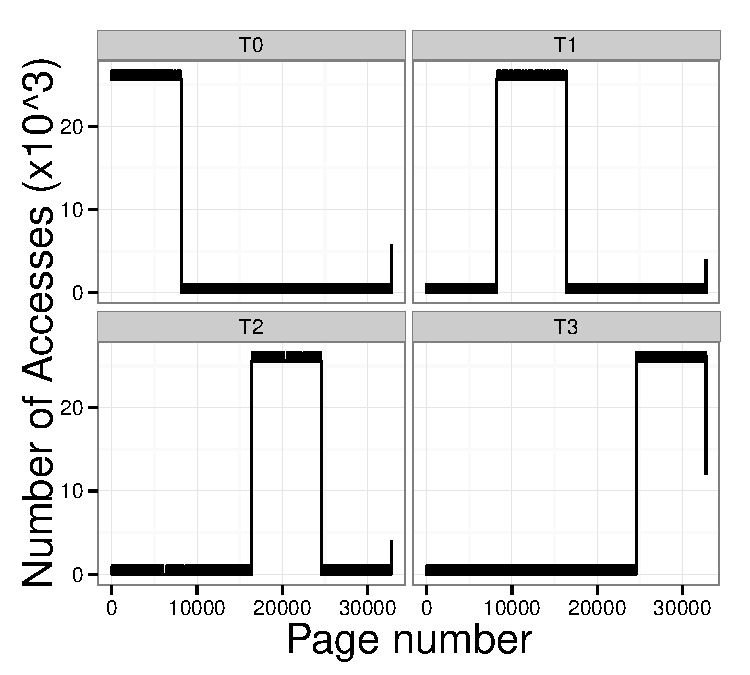
\includegraphics[height=.2\textheight]  {is_w_kba_orig}
        \label{fig:is-behaviour-orig-kba}
    }
    \vspace{-1mm}
    \subfigure[\texttt{key\_buff1}.]{
        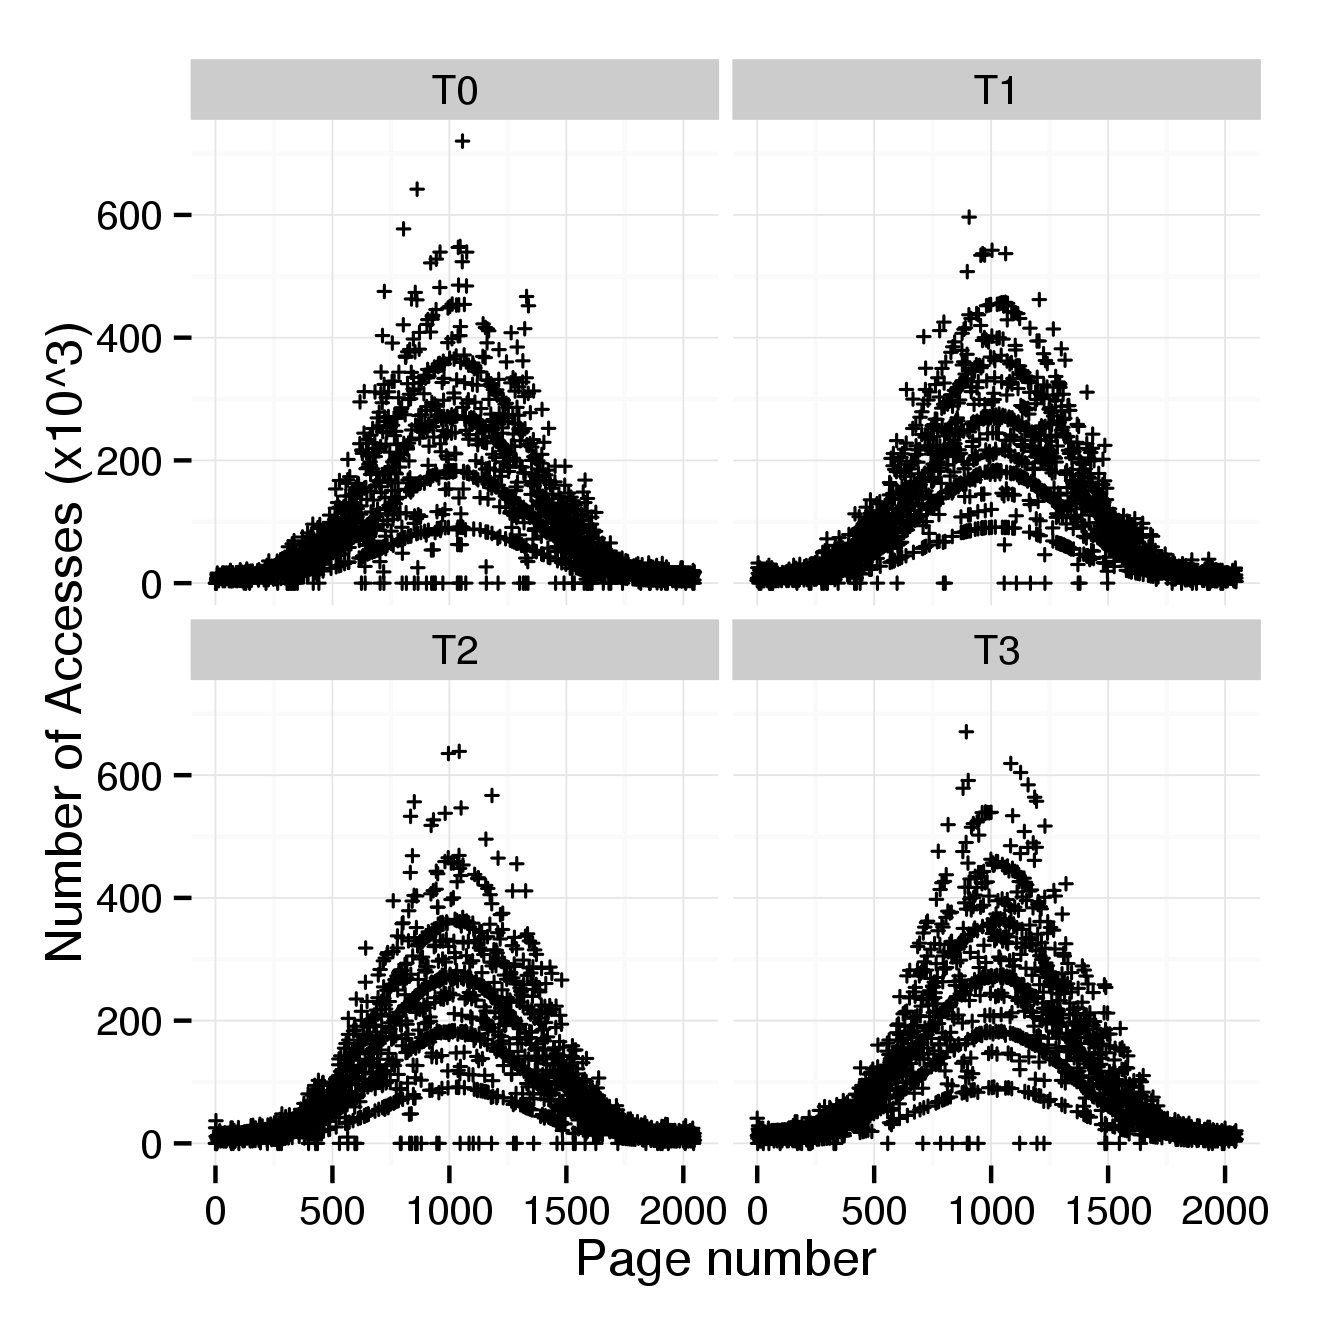
\includegraphics[height=.2\textheight]  {is_w_kb1_orig}
        \label{fig:is-behaviour-orig-kb1}
    }
    \caption{Original memory access distribution for the main structures of
        \emph{IS} with $4$ threads.}
    \label{fig:is-behaviour-orig}
\end{figure}
Figure~\ref{fig:is-behaviour-orig} shows the access distributions for the
three main structures of \emph{IS} class \emph{W} with $4$ threads. We can see that
each structure has a different access pattern: \texttt{key\_array}'s
(Figure~\ref{fig:is-behaviour-orig-kba}) access distribution shows that every
thread works on a different part of the structure, which allows automated
tools to perform an efficient data/thread mapping on it. On the other hand, \texttt{key\_buff2}
(Figure~\ref{fig:is-behaviour-orig-kb2}) is completely shared by all threads.
The most interesting access distribution is the one of \texttt{key\_buff1}
(Figure~\ref{fig:is-behaviour-orig-kb1}). The access distribution follows a clear Gaussian curve, which means that a few pages are more used than the
others. With such a distribution, automated tools might generate a lot of page
migrations.

\lstinputlisting[caption=\emph{IS} code responsible for the
Gaussian distribution of memory accesses to the \texttt{key\_buff1} structure., label=lst:is, float=!p]{code/is.c}

With this knowledge, we can identify the source of the
Gaussian pattern in the \emph{IS} source code. All the accesses to \texttt{key\_buff1} are linear,
except the ones shown in Listing~\ref{lst:is}\footnote{
    The code has been slightly modified to make it more readable. In the
    original version, the arrays \texttt{key\_buff1} (resp. \texttt{key\_buff2})
    are accessed via a generic pointer called \texttt{key\_buff\_ptr} (resp.
    \texttt{key\_buff\_ptr2}).
}, line \ref{lst:is-gaus-end}, which depend on the values of
\texttt{key\_buff2}.
By default, OpenMP threads are scheduled dynamically to avoid unbalanced
distribution of work, but the developers also propose a cyclic distribution
of the threads over the loop. As we know that the value of \texttt{key\_buff2}
follows a Gaussian distribution, we can design a distribution of the threads
providing both a good load balancing and locality of data. To do so, we split
the loop into two parts and distribute each part over the threads in a round-robin way. This can be done by modifying line \ref{lst:is-sched} of the original code, as shown
in Listing~\ref{lst:is-modif}.

\begin{lstlisting}[float=!ht,caption=Optimization for \emph{IS}., label=lst:is-modif]
#pragma omp for schedule(static,NUM_BUCKETS/(2*omp_get_max_threads()))
\end{lstlisting}

\begin{figure}[!p]
    \centering

    \subfigure[The \texttt{key\_buff2} structure.]{
        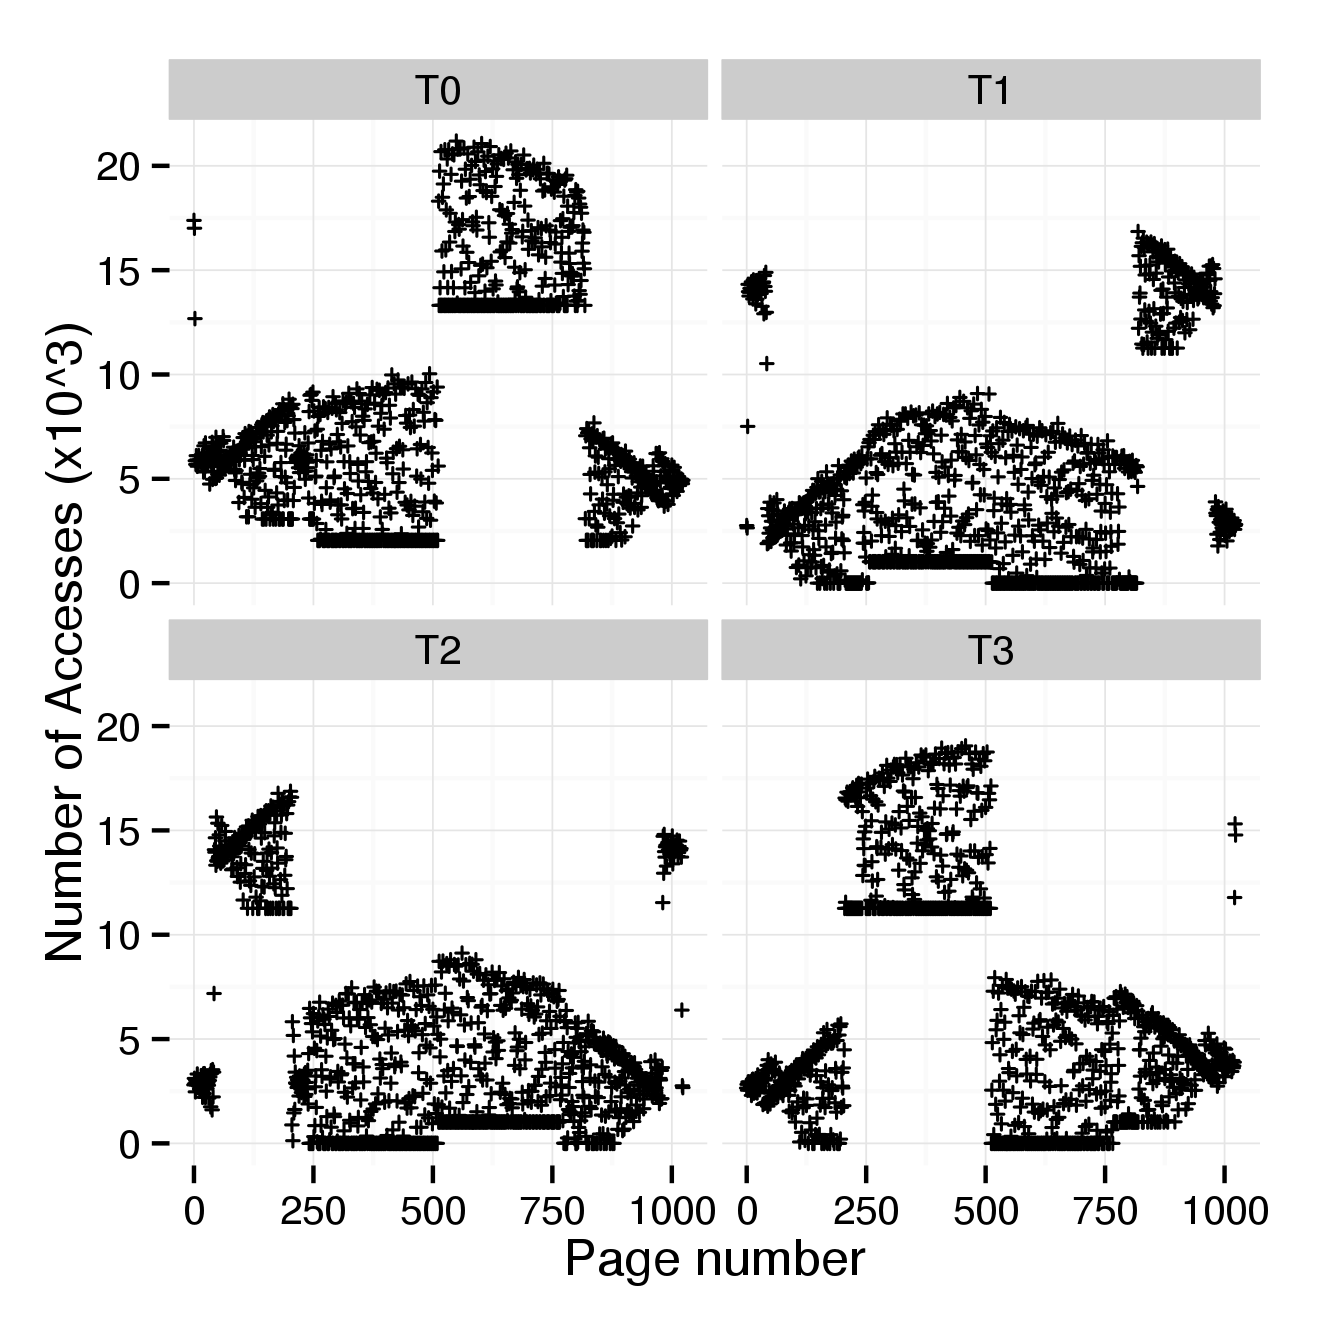
\includegraphics[height=.2\textheight] {is_w_kb2_modif}
        \label{fig:is-behaviour-modif-kb2}
    }

    \vspace{-3mm}
    \subfigure[The \texttt{key\_array} structure.]{
        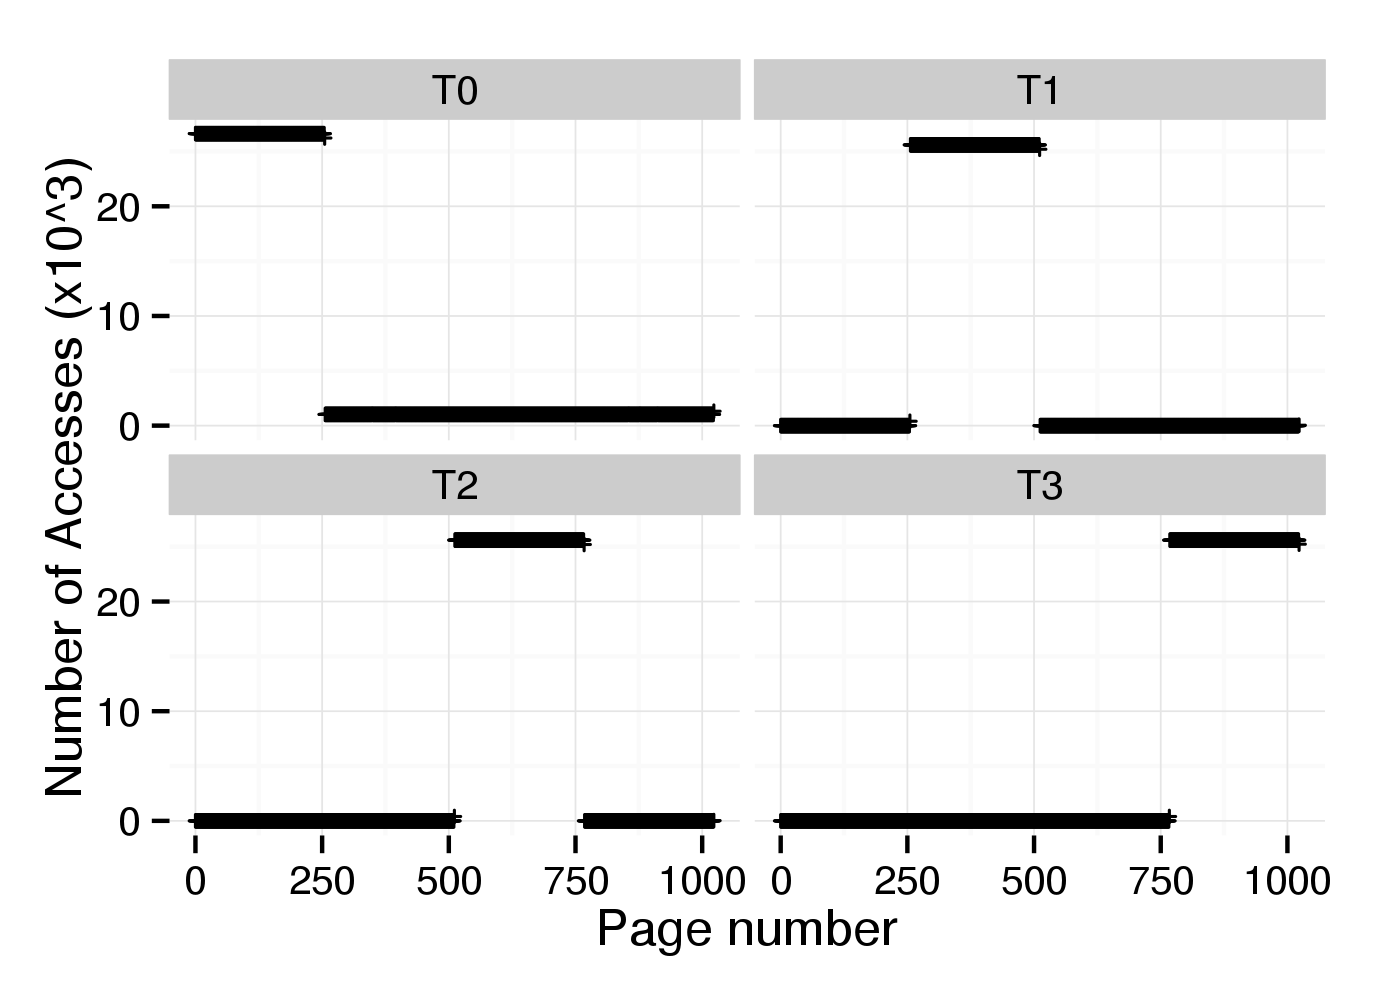
\includegraphics[height=.2\textheight] {is_w_kba_modif}
        \label{fig:is-behaviour-modif-kba}
    }

    \vspace{-3mm}
    \subfigure[The \texttt{key\_buff1} structure.]{
        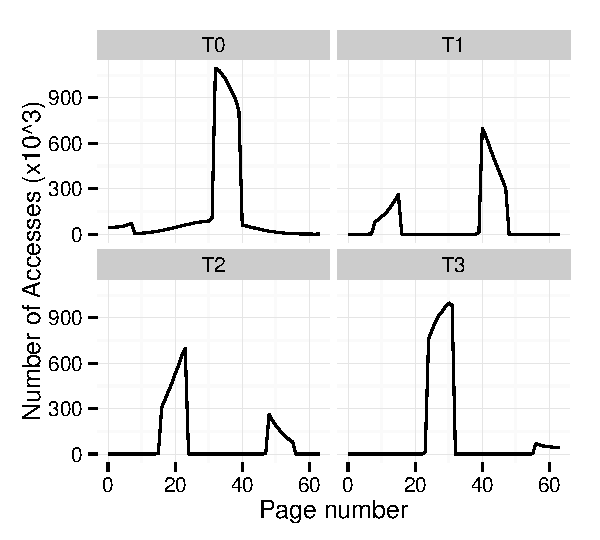
\includegraphics[height=.2\textheight] {is_w_kb1_modif}
        \label{fig:is-behaviour-modif-kb1}
    }

    \vspace{-3mm}
    \caption{Memory access distribution for the main structures of
        \emph{IS} with $4$ threads after our modifications.}
    \label{fig:is-behaviour-modif}
\end{figure}


With this simple code modification, we obtain the access distribution
shown in Figure~\ref{fig:is-behaviour-modif}. We can see that the Gaussian
access pattern of \texttt{key\_buff1} is now distributed between the threads. Each page
of this structure is mostly used by only one thread. Moreover,
\texttt{key\_buff2}'s access distribution has also changed. We can see that
each thread uses mostly one part of the array.
The main point of our code modification is to improve the affinity between
thread and memory, therefore we need to pin each thread on a core to keep them
near to their data. To perform the mapping, we use the \texttt{GOMP\_CPU\_AFFINITY} environment variable. \TABARNAC
also shows us that the first touch is always done by the thread actually using
the data for IS, therefore we do not need to map the data to the NUMA nodes.

We then compare the execution time of \emph{IS} (class \emph{D}) for the three scheduling
methods, \emph{Dynamic}, \emph{Cyclic} with a step of $1$ and \TABARNAC:
cyclic with the proposed distribution. For the two first methods, we compare the
execution time on the bare operation system (Base), the execution time with an
interleave policy (Interleave) and with NUMA balancing enabled in the kernel
(NUMA Balancing). Interleave and NUMA Balancing are not relevant with
\TABARNAC modifications and are therefore not shown.

\begin{figure}[!p]
    \centering
    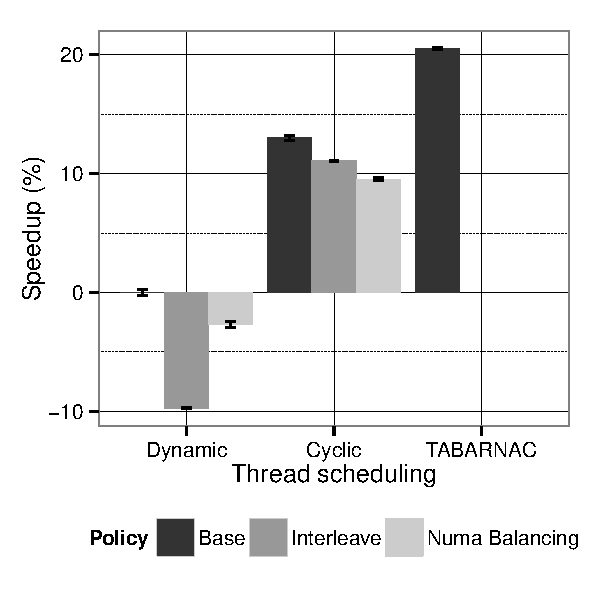
\includegraphics[width=.7\linewidth]{is_exectime}
    \vspace{-5mm}
    \caption{Speedup for \emph{IS} (class D) compared to the baseline.}
\label{fig:is-res}
\end{figure}

Figure~\ref{fig:is-res} shows the speedup of \emph{IS} compared to
the default version (\emph{Dynamic}) for each scheduling method and for each
optimization technique. The first thing to notice is that with the default
\emph{Dynamic} scheduling, both Interleave and NUMA Balancing slow
the application down, by up to $10\%$. This shows that simple, automatic optimization policies are can actually reduce performance
for non NUMA conscious code.
The \emph{Cyclic} policy, proposed in the original code, already provides up to $13\%$
speedup. We can see that both interleave and NUMA Balancing are not suitable
for this policy, since they reduce the performance gains.
The \TABARNAC version provides more than $20\%$ speedup with very small code
modification.
This example shows how analyzing an application's memory behavior can lead to
significant execution time improvement where automatic tools can actually slow
the application down.

\subsection{Ondes3D}
\label{sec:exp-ondes3d}

\begin{figure}[!t]
    \centering

    \subfigure[Access distribution for \texttt{fz}.]{
        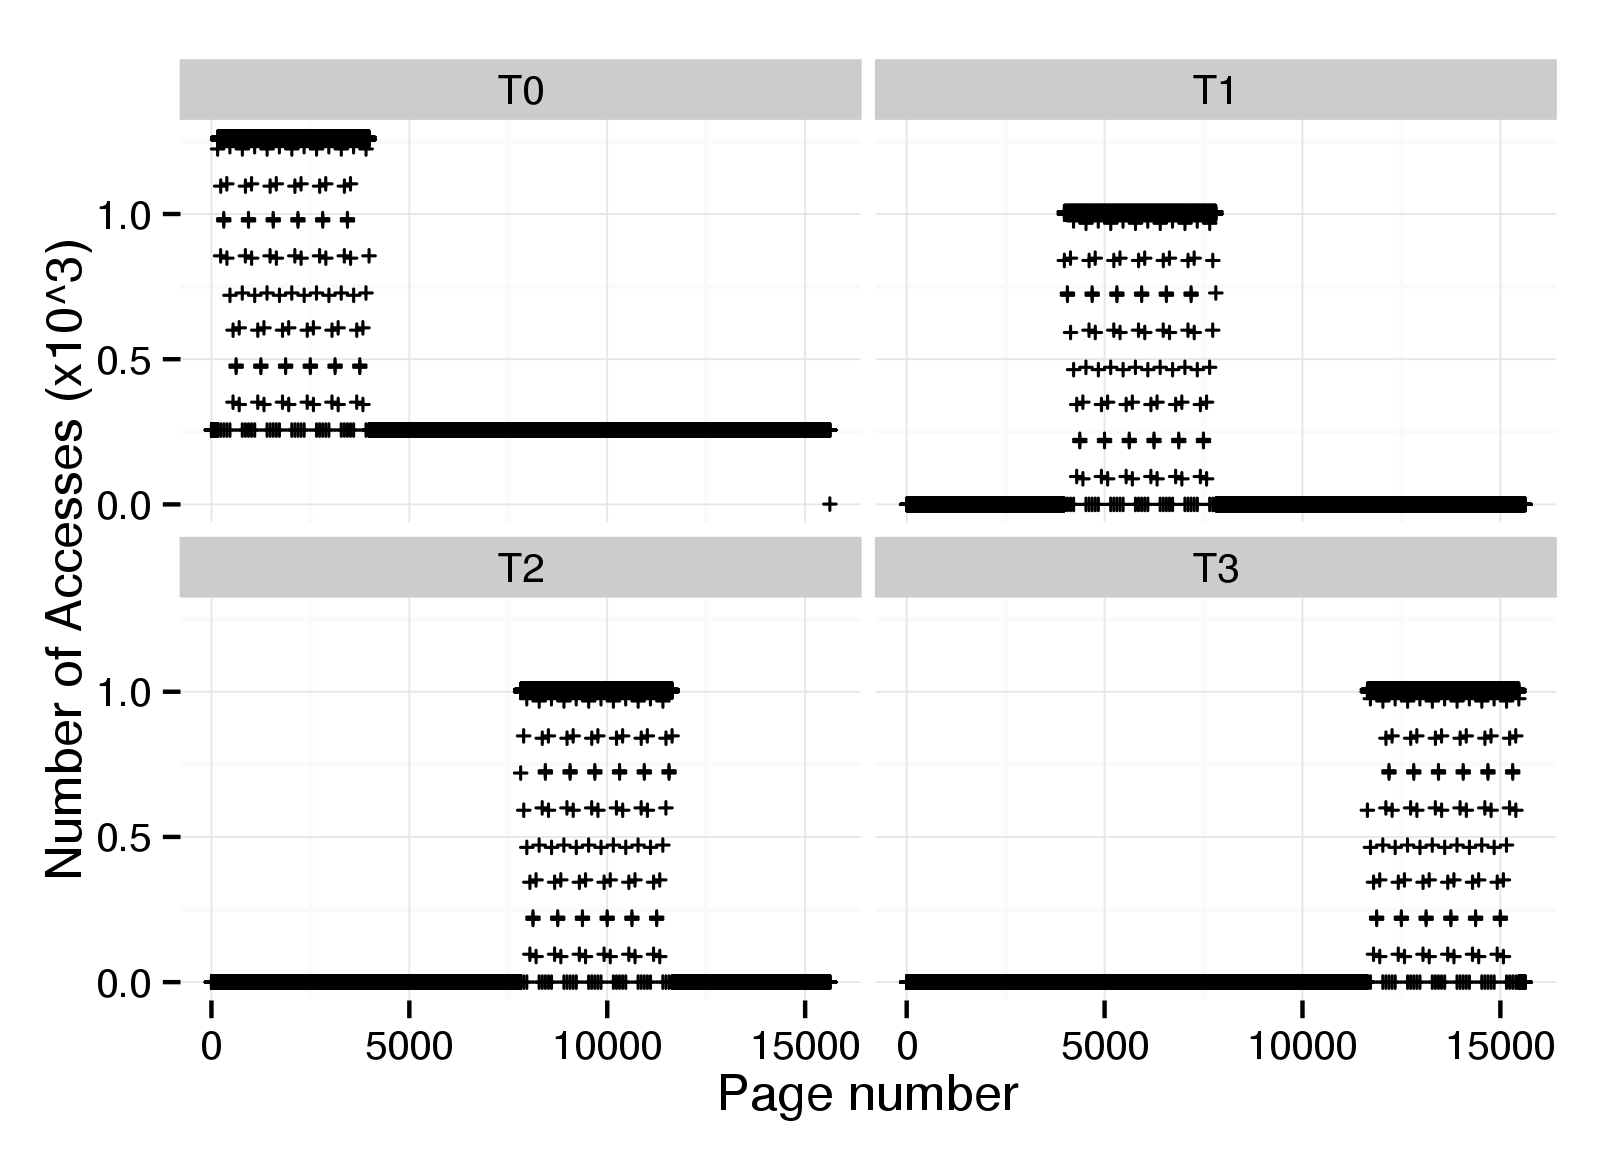
\includegraphics[height=.24\textheight] {ondes3d_fz_dist_orig}
        \label{fig:ondes3d-behaviour-fz-orig}
    }
    \subfigure[First-touch \texttt{fz}.]{
        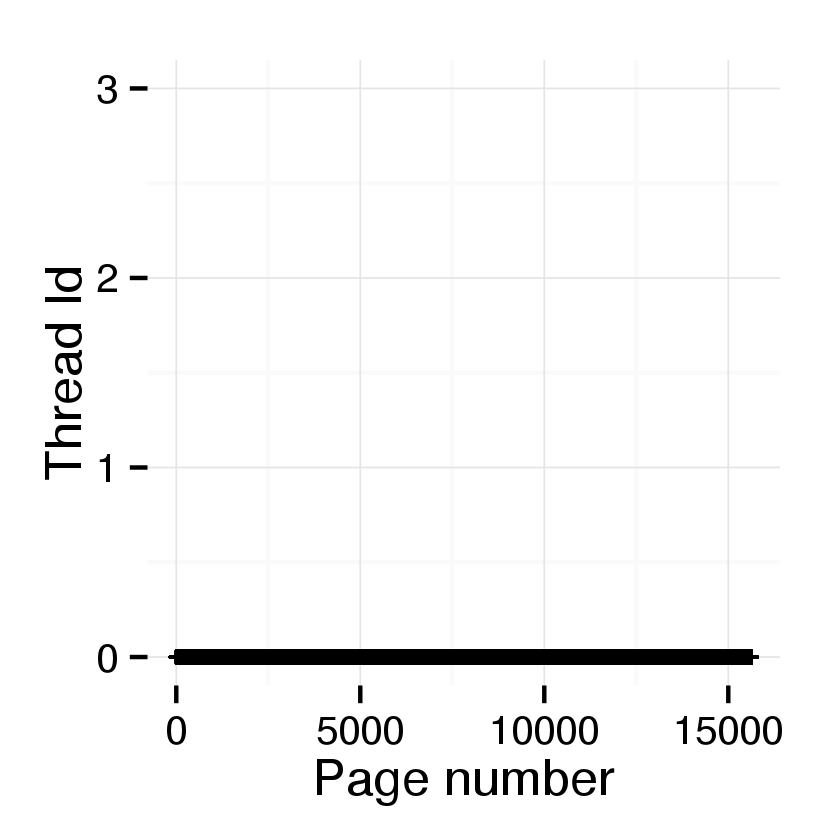
\includegraphics[height=.24\textheight] {ondes3d_fz_ft_orig}
        \label{fig:ondes3d-ft-fz-orig}
    }
    \caption{Original access and first-touch distribution for structure
        \texttt{fz} from \emph{Ondes3D}.}
    \label{fig:ondes3d-orig}
\end{figure}

The analysis of \emph{Ondes3D} access distributions shows that each
structure is well divided between the threads, as we can see for structure \texttt{fz} in Figure~\ref{fig:ondes3d-behaviour-fz-orig}.
However, we note that thread $T0$ seems to access the whole structure. By looking at the first touch distribution (Figure~\ref{fig:ondes3d-ft-fz-orig}), we
notice that indeed this thread is responsible for all first accesses to this structure. Due to
this pattern, if we run \emph{Ondes3D} without any mapping, every page
will be mapped to the NUMA node that executes $T0$, resulting in many remote accesses for the other threads. An easy fix is to
perform the initialization in parallel and to pin each thread on a different core.

\begin{figure}[!t]
    \centering

    \subfigure[Access distribution for \texttt{fz}.]{
        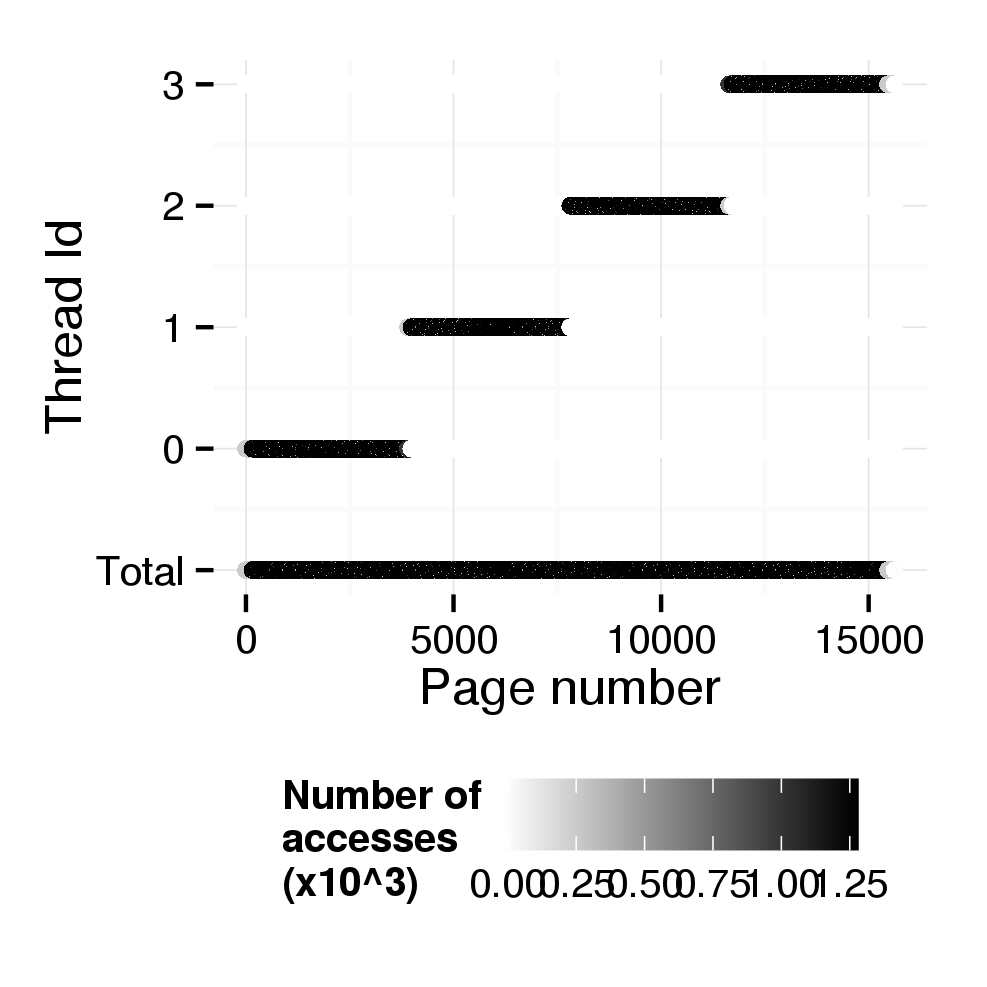
\includegraphics[height=.24\textheight] {ondes3d_fz_dist_modif}
        \label{fig:ondes3d-behaviour-fz-modif}
    }
    \subfigure[First-touch \texttt{fz}.]{
        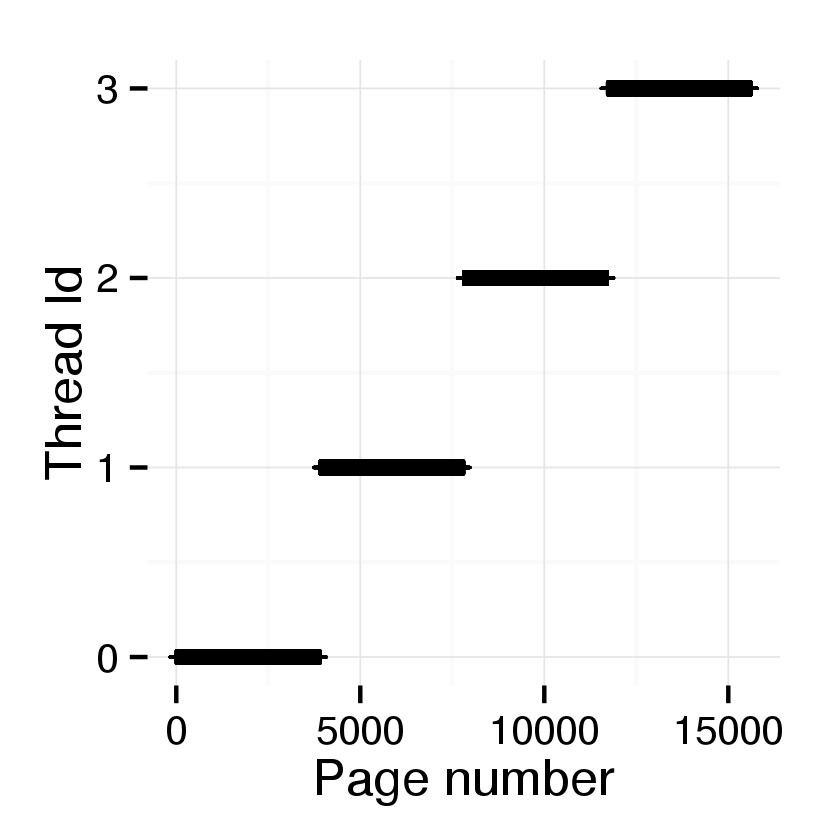
\includegraphics[height=.24\textheight] {ondes3d_fz_ft_modif}
        \label{fig:ondes3d-ft-fz-modif}
    }
    \caption{Access and first-touch distribution  for structure
        \texttt{fz} from \emph{Ondes3D}, after modifications.}
    \label{fig:ondes3d-modif}
\end{figure}

Such modifications result in the access distribution shown in Figure~\ref{fig:ondes3d-behaviour-fz-modif}. We can see that now $T0$ accesses only
its own portion of the structure. Moreover, Figure~\ref{fig:ondes3d-ft-fz-modif} shows that the first touch is now distributed
over the structures and matches the actual access distribution, as expected.

\begin{figure}[!t]
    \centering
    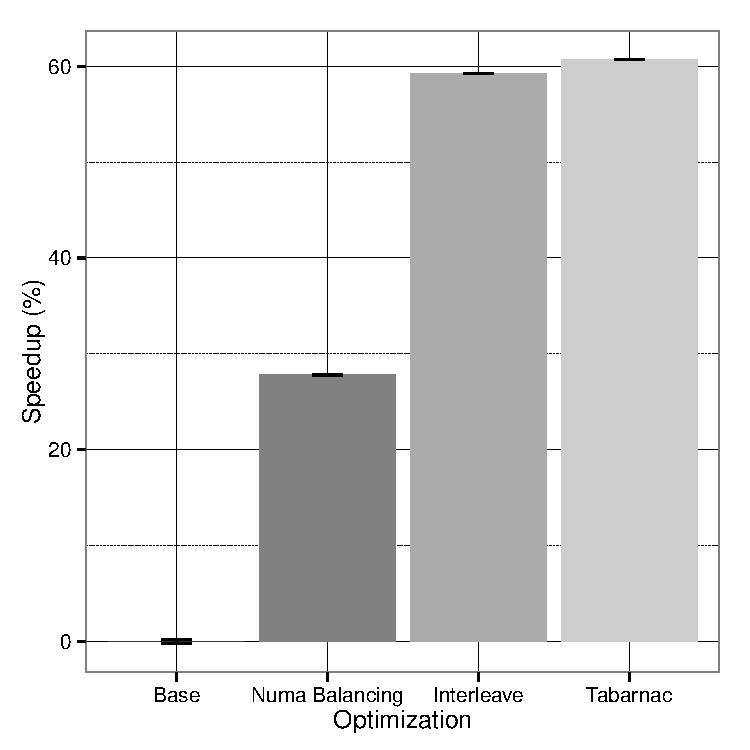
\includegraphics[width=.7\linewidth]{ondes3d_exectime}
    \caption{Speedup for \emph{Ondes3D} compared to the original application.}
\label{fig:ondes-res}
\end{figure}

We evaluate the modified version by comparing it with the original
version, running on the normal OS, with NUMA Balancing activated and with an
interleave policy. Figure~\ref{fig:ondes-res} present the results of this
evaluation. We can see that every method improves the execution time, but
NUMA Balancing provides less than $30\%$ speedup, while the static mapping
(Interleave or the modified code) allows us to get almost $60\%$ of speedup. This is
due to the training time described in section \ref{sec:soa-mapping}. Indeed,
with NUMA Balancing, all pages are initially mapped by the OS to the NUMA node of thread $T0$, they
are only moved a while later, after many remote accesses have already occurred. This is a case where static mapping can be substantially better than automated
tools. \tod{remove?:} The Interleave policy provides almost the same speedup as
\TABARNAC as it distributes the pages over the NUMA nodes at the beginning of
the execution.
% Nevertheless, the interleave version only maps the data no the
% threads, therefore if the performances might drop if the OS does not map them
% ``correctly'' while the modified version proposes a thread mapping that ensures better
% data locality.

\subsection{Analysis Overhead}
\label{sec:expe-overhead}

Our last experiment aims at evaluating the instrumentation cost. To evaluate the analysis overhead of \TABARNAC, we
executed all the NAS Parallel Benchmarks in class B with 64 threads and compared
the original execution time with the execution time under instrumentation.

\begin{figure}[!t]
    \centering
    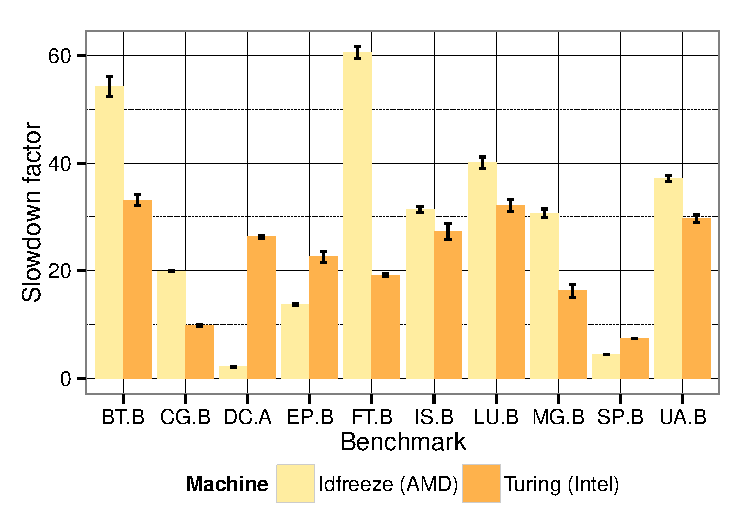
\includegraphics[width=.7\linewidth]{tool-ovh.pdf}
    \caption{Overhead of \TABARNAC analysis for the NAS Parallel Benchmarks.}
    \label{fig:ovh}
\end{figure}


We can see in Figure~\ref{fig:ovh} that
the instrumentation is $10$ to $30$ times slower than the normal execution. Although it is
not negligible, we have to consider the fact that often we can instrument
smaller versions of the applications, as we focus on the general behavior.
Moreover, as we do not use sampling, our instrumentation is deterministic and
there is no need to run the instrumentation several times. Finally, as our
analysis is designed to be used during the development phase of the
application and not by an automated tool during the execution, even a factor of $30$
can be reasonable.

\subsection{Summary}

\tod{write this}

- automatic policies with deficits (slower compared to baseline in many cases)

- \TABARNAC always highest improvements

- simple applications changes/mappings can result in substantial improvements

- correct policy depends on application
